
%(BEGIN_QUESTION)
% Copyright 2009, Tony R. Kuphaldt, released under the Creative Commons Attribution License (v 1.0)
% This means you may do almost anything with this work of mine, so long as you give me proper credit

Read and outline the ``Lag Time Compensation'' subsection of the ``Feedforward with Dynamic Compensation'' section of the ``Basic Process Control Strategies'' chapter in your {\it Lessons In Industrial Instrumentation} textbook.  Note the page numbers where important illustrations, photographs, equations, tables, and other relevant details are found.  Prepare to thoughtfully discuss with your instructor and classmates the concepts and examples explored in this reading.

\underbar{file i04342}
%(END_QUESTION)





%(BEGIN_ANSWER)


%(END_ANSWER)





%(BEGIN_NOTES)

Lag time is the amount of time a process takes to go 63.2\% of the way from its initial value to its final value ($\tau$).  Sometimes we see feedforward applications where the feedforward corrective action has a different lag time than the load does.  If these lag times are unequal, feedforward compensation will temporarily over- or under-compensate.

\vskip 10pt

In our example of an oil preheating exchanger, the dominant load is cold oil feed rate.  Measuring this feed rate and using it as a feedforward signal to the steam valve helps the feedback control system achieve better stability when the feed rate quickly changes.  In this system, changes in oil flow rate have a {\it faster} effect on outlet temperature than changes in steam flow rate.  Therefore, feedforward tends to under-compensate for a brief period of time because the feedforward correction lags behind the load's effect.

\vskip 10pt

We may help equalize time lags by intentionally installing lead/lag function blocks in the feedforward signal path.  Lag functions will add to lag time, while lead functions subtract from lag time.

\vskip 10pt

With a lead function block installed in the feed flow signal path, the exchanger's steam valve will momentarily ``surge'' in such a way that it speeds up the response of the steam to help reduce that time lag, so that the feedforward action takes effect at approximately the same time as the effect of the oil flow change.









\vskip 20pt \vbox{\hrule \hbox{\strut \vrule{} {\bf Suggestions for Socratic discussion} \vrule} \hrule}

\begin{itemize}
\item{} Explain how lag time differs from dead time.
\item{} Explain how the simple heat exchanger feedforward system failed to produce perfect results.
\item{} Explain why the addition of a {\it lead} function was necessary to help the heat exchanger's feedforward system produce better results.
\item{} Explain how we determined a {\it lead} function was necessary in the feedforward signal path rather than a {\it lag} function.
\item{} Describe a procedure by which you would empirically determine the right amount of lead to put into the lead function block in this system.
\end{itemize}









\vfil \eject

\noindent
{\bf Summary Quiz:}

The {\it lead} function block is included in this feedforward control system because:

$$\includegraphics[width=15.5cm]{i04342x01.eps}$$

\begin{itemize}
\item{} It just looks cool sitting there like it belongs 
\vskip 10pt 
\item{} The process temperature responds more slowly to changes in cold oil flow than to changes in steam flow 
\vskip 10pt 
\item{} The control valve is ``sticky'' and needs help overcoming the hysteresis of packing friction
\vskip 10pt 
\item{} The process temperature responds more slowly to changes in steam flow than to changes in cold oil flow
\vskip 10pt 
\item{} The steam flow transmitter has too much damping (lag) that must be compensated for
\vskip 10pt 
\item{} The temperature controller lacks derivative response, which would be helpful for this process
\end{itemize}

%INDEX% Reading assignment: Lessons In Industrial Instrumentation, basic control strategies (feedforward w/ lag time compensation)

%(END_NOTES)


